% Appendices are set up same as chapters
% \chapter{Moderator Prototype Data}
% \label{sec:Appendix1}
% Adapted from Autodesk Fall 2007-08 \cite{Autodesk2008Fall}.

% \begin{figure}
%       \centering
%               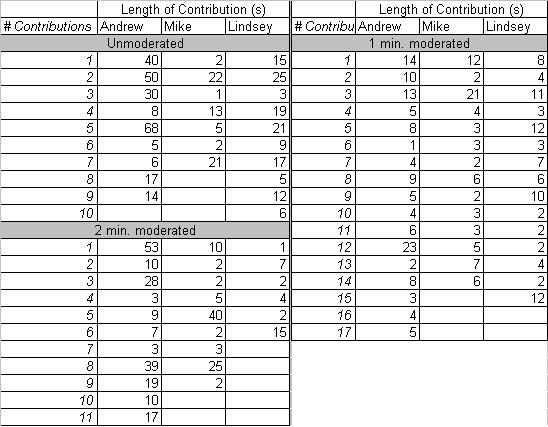
\includegraphics[width=0.75\textwidth]{Figures/Appendix1/moderatordata.JPG}
%               %Note the use of a short caption tag for the list of figures.
%       \caption[test meetings data]{Length and number of contributions collected from recorded moderator test meetings}
%       \label{fig:moderatordata}
% \end{figure}
\chapter{CC BY-SA 3.0 License}
\subsection*{Attribution-ShareAlike 3.0 Unported  (CC BY-SA 3.0) }
Disclaimer

  The Commons Deed is not a license. It is simply a handy reference for understanding the Legal Code (the full license) — it is a human-readable expression of some of its key terms. Think of it as the user-friendly interface to the Legal Code beneath. This Deed itself has no legal value, and its contents do not appear in the actual license. 


  Creative Commons is not a law firm and does not provide legal services. Distributing of, displaying of, or linking to this Commons Deed does not create an attorney-client relationship. 
 This is a human-readable summary of the Legal Code (the full license).  Disclaimer  This license is acceptable for Free Cultural Works. \subsubsection*{You are free:}
\begin{itemize}
\item \textbf{to Share}
--- to copy, distribute and transmit the work 
\item \textbf{to Remix}
--- to adapt the work 
\item  to make commercial use of the work 

\end{itemize}
\subsubsection*{Under the following conditions:}
\begin{itemize}
\item 

 \textbf{Attribution}
 ---  You must attribute the work in the manner specified by the author or licensor (but not in any way that suggests that they endorse you or your use of the work).   


%  \textbf{ Attribute this work: }
% \\ 
%     Information 
%  What does ``Attribute this work'' mean?  The page you came from contained embedded licensing metadata, including how the creator wishes to be attributed for re-use. You can use the HTML here to cite the work. Doing so will also include metadata on your page so that others can find the original work as well. 
\item 

 \textbf{Share Alike}
 --- If you alter, transform, or build upon this work, you may distribute the resulting work only under the same or similar license to this one.  


\end{itemize}
\subsubsection*{ With the understanding that: }
\begin{itemize}
\item \textbf{Waiver}
 --- Any of the above conditions can be waived if you get permission from the copyright holder. 
\item \textbf{Public Domain}
 --- Where the work or any of its elements is in the public domain under applicable law, that status is in no way affected by the license. 
\item \textbf{Other Rights}
 --- In no way are any of the following rights affected by the license: \begin{itemize}
\item  Your fair dealing or fair use rights, or other applicable copyright exceptions and limitations; 
\item  The author's moral rights; 
\item  Rights other persons may have either in the work itself or in how the work is used, such as publicity or privacy rights. 

\end{itemize}
\end{itemize}
